\documentclass{beamer}
\usepackage{Presentacion}

\title[Detección de Deadlocks en Rust]{Detección de Deadlocks en Rust \\ en tiempo de compilación \\ mediante Redes de Petri}
\author{Horacio Lisdero Scaffino}
\institute[FIUBA]{Facultad de Ingeniería\\Universidad de Buenos Aires}
\date{19 de febrero del 2023}
% TWEAK THE FONT SIZE
\setbeamerfont{date}{size=\scriptsize}
% ADD LOGO
\logo{
\includegraphics[height=1.3cm]{FIUBA-Logo.png}}

\AtBeginSection[]
{
  \begin{frame}{Agenda}
  \footnotesize
    \tableofcontents[currentsection, currentsubsection]
  \end{frame}
}

\AtBeginSubsection[]
{
  \begin{frame}{Agenda}
  \footnotesize
    \tableofcontents[currentsection, currentsubsection]
  \end{frame}
}

\begin{document}

\begin{frame}
  \titlepage
\end{frame}

% REMOVE THE LOGO FROM NOW ON %
\logo{}

\begin{frame}{Agenda}
  \tableofcontents
\end{frame}

\section{Introducción}

\begin{frame}{Una vista general de la herramienta}
  El traductor es el componente principal.
  El verificador de modelos y el compilador de Rust, \emph{rustc}, son dependencias.

  \begin{figure}
    \centering
    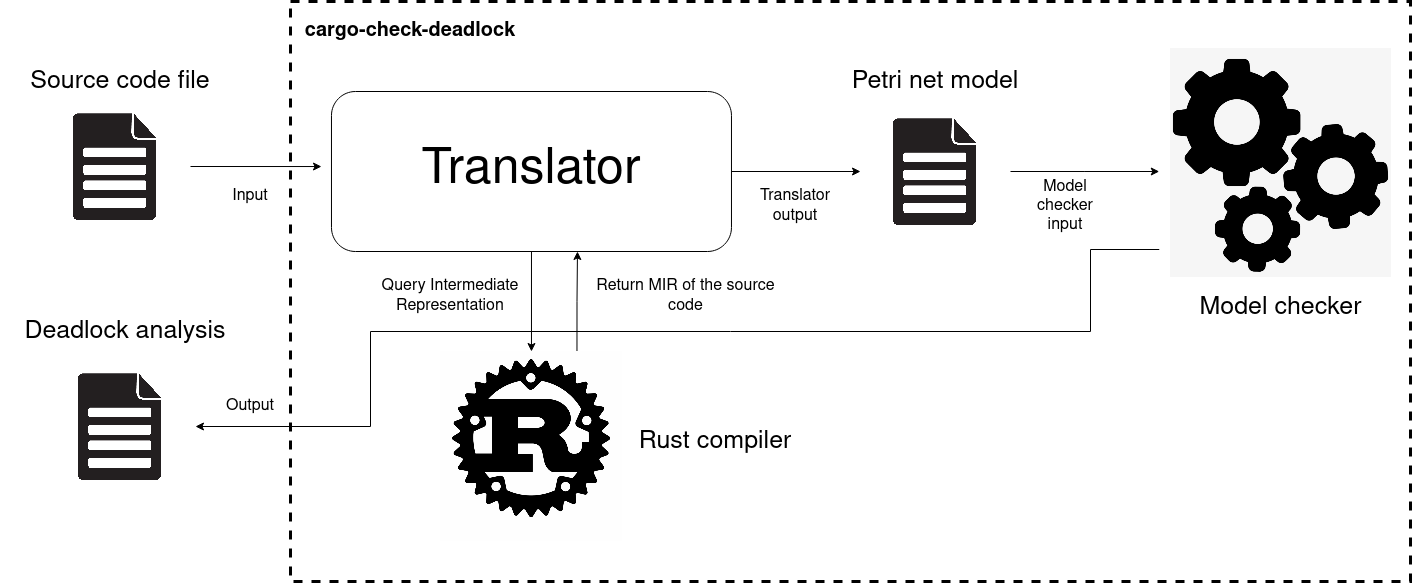
\includegraphics[width=\linewidth]{cargo-check-deadlock-logic-view.png}
  \end{figure}
\end{frame}

\section{Rust}

\subsection{¿Qué es Rust?}

\begin{frame}{¿Qué es Rust?}
  Rust es un lenguaje de programación multiparadigma de uso general que
  busca ofrecer a los desarrolladores una forma segura y eficiente de escribir código de bajo nivel.
  
  \pause
  \vfill

  \begin{itemize}
    \item Uso seguro de la memoria (\emph{Memory safe})
    \item Compilado a código máquina, con un \emph{runtime} mínimo
    \item Expresividad de un lenguaje de alto nivel
    \item Performance de un lenguaje de bajo nivel (similar a C o C++)
  \end{itemize}
\end{frame}

\begin{frame}{Breve línea de tiempo de Rust}
  \begin{description}
    \item [2007] Inicio como un proyecto personal de Graydon Hoare, un programador en Mozilla
    \item [2009] Mozilla comienza a patrocinar oficialmente el proyecto
    \item [2015] Primera versión estable 1.0
    \item [2016] Mozilla lanza Servo, un motor de navegador construido con Rust
    \item [2019] Se estabiliza el soporte de \Rustinline{async}/\Rustinline{await}
    \item [2021] AWS, Huawei, Google, Microsoft y Mozilla crean la Rust Foundation.
    \item [2021] El proyecto Android fomenta el uso de Rust para los componentes del SO por debajo del ART
    \item [2022] El kernel de Linux añade soporte para Rust junto con C
    \item [2023] 8 años consecutivos el lenguaje de programación más querido en la Stack Overflow Developer Survey
  \end{description}
\end{frame}

\begin{frame}{Uso seguro de la memoria}
  Logra un uso seguro de la memoria sin recurrir a un recolector de basura o a un contador de referencias.
  En su lugar, utiliza el concepto de \textbf{ownership} (propiedad) y \textbf{borrowing} (préstamo).

  \vfill

  Evita una gran variedad de clases de errores en tiempo de compilación:

  \begin{itemize}
    \item Double free
    \item Use after free
    \item Punteros colgantes (\emph{Dangling pointers})
    \item Condiciones de carrera (\emph{Data races})
    \item Pasaje de variables no seguras entre hilos
  \end{itemize}

  \vfill

  Si se encuentra una violación de las reglas del compilador, el programa simplemente no compilará.
\end{frame}

\subsection{¿Por qué Rust?}

\begin{frame}{El uso seguro de la memoria es fundamental para la fiabilidad y la seguridad}
  Investigaciones empíricas han concluido que alrededor del 70\% de las vulnerabilidades encontradas en
  grandes bases de código en C/C++ se deben a errores de gestión de memoria.
  Esta elevada cifra puede observarse en proyectos como:

  \begin{itemize}
    \item Android Open Source Project \cite{memory-bugs-android},
    \item los componentes Bluetooth y multimedia de Android \cite{memory-bugs-android-media-bluetooth},
    \item el Proyecto Chromium detrás del navegador web Chrome \cite{memory-bugs-chrome},
    \item el componente CSS de Firefox \cite{memory-bugs-firefox},
    \item iOS y macOS \cite{memory-bugs-ios-macos},
    \item productos de Microsoft \cite{miller-security-microsoft2019, memory-bugs-microsoft},
    \item Ubuntu \cite{memory-bugs-ubuntu}
  \end{itemize}
\end{frame}

\begin{frame}{La adopción de Rust aumenta velozmente}
  \scriptsize
  \begin{itemize}
    \item El proyecto Android Open Source fomenta
          el uso de Rust para los componentes del SO
          por debajo del ART \cite{stoep2021}.
    \item El kernel Linux versión 6.1 introduce soporte oficial de las herramientas
          para programar componentes en Rust \cite{corbet2022,desimone2022}.
    \item En Mozilla, el proyecto Oxidation se creó en 
          para aumentar el uso de Rust en Firefox y aplicaciones relacionadas. 
          En marzo de 2023, las líneas de código en Rust representan
          más del 10\% del total en Firefox Nightly \cite{mozilla-oxidation}.
    \item En Meta, el uso de Rust como lenguaje de desarrollo \emph{server-side}
          está aprobado y se fomenta desde julio de 2022 \cite{garcia2022}.
    \item En Cloudflare, se construyó desde cero un nuevo proxy HTTP en Rust
          para superar las limitaciones arquitectónicas de NGINX,
          reduciendo el uso de CPU en un 70\% y el uso de memoria en un 67\% \cite{wu2022}.
    \item En Discord, reimplementar un servicio crucial
          en Rust proporcionó grandes beneficios de performance
          y solucionó un problema ligado a la recolección de basura en Go \cite{howarth2020}.
    \item En npm Inc, la empresa detrás del registro npm,
          Rust permitió escalar los servicios ligados a la CPU
          a más de 1300 millones de descargas diarias \cite{rust-npm-case-study}.
    \item Un estudio del código basado en Rust descubrió que se ejecuta tan eficientemente
          que consume la mitad de electricidad que un programa similar escrito en Java,
          un lenguaje de uso común en AWS \cite{pereira2017energy}.
  \end{itemize}
\end{frame}

\begin{frame}{Las herramientas son modernas y fáciles de usar}
  \begin{itemize}
    \item \href{https://doc.rust-lang.org/stable/cargo/}{cargo},
          el gestor de paquetes oficial: Formatear, compilar, testear, lint, actualizar y publicar paquetes.
    \item \href{https://doc.rust-lang.org/book/ch11-00-testing.html}{Test harness}
          para pruebas unitarias, pruebas de integración y pruebas en comentarios de documentación (doctests).
          No se necesitan bibliotecas de terceros.
    \item Un registro público oficial para los paquetes Rust (llamados ``crates''): \url{https://crates.io/}.
    \item Generación automática de un sitio web estático a partir de los comentarios en el código del proyecto.
          Se publica automáticamente en \url{https://docs.rs/}.
    \item Un linter oficial incluido en la instalación por defecto que detecta aún más errores
          y detecta código no idiomático: \href{https://github.com/rust-lang/rust-clippy}{clippy}.
    \item La integración con git, GitHub, VSCode, IntelliJ es excelente y fácil de usar.
    \item Una nueva versión estable del compilador cada 6 semanas \cite{albini2019}.
  \end{itemize}
\end{frame}

\section{Redes de Petri}

\subsection{¿Qué es una red de Petri?}

\begin{frame}{Definición informal}
  Una red de Petri es una herramienta de modelado matemático
  utilizada para describir y analizar el comportamiento de sistemas concurrentes.
  Proporciona una representación gráfica del estado del sistema y sus transiciones,
  permitiendo el análisis visual y formal de procesos complejos.

  \begin{figure}[!htb]
    \centering
    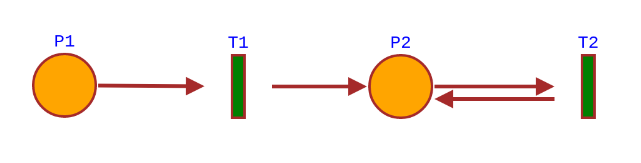
\includegraphics[width=0.8\linewidth]{petri-net-formal-example.png}
  \end{figure}

  \scriptsize
  \begin{itemize}
    \item Lugares: Representan estados en el sistema (\emph{circles})
    \item Transiciones: Representan eventos o acciones que ocurren en el sistema (\emph{rectángulos}).
    \item Tokens: Marcas dentro de lugares que son creadas
          y consumidas por las transiciones (\emph{puntos dentro de lugares})
  \end{itemize}

  \vfill
\end{frame}

\begin{frame}{Definición matemática}
  Una red de Petri es una 5-tupla, $ PN = (P, T, F, W, M_{0}) $ donde:

  \begin{quote}
    $ P = \{ p_1, p_2, \dots, p_m \} $ es un conjunto finito de lugares,\\
    $ T = \{ t_1, t_2, \dots, t_n \} $ es un conjunto finito de transiciones,\\
    $ F \subseteq (P \times T) \cup (T \times P) $ es un conjunto de arcos (relación de flujo),\\
    $ W: F \rightarrow \{1, 2, 3, ... \} $ es una función de peso para los arcos,\\
    $ M_{0}: P \rightarrow \{0, 1, 2, 3, .... \} $ es el marcado inicial,\\
    $ P \cap T = \varnothing $ y $ P \cup T \neq \varnothing $
  \end{quote}
  
  \vfill

  El grafo es por definición \emph{bipartito}.
  Solo puede haber aristas:
  \begin{itemize}
    \item de lugares a transiciones
    \item de transiciones a lugares
  \end{itemize}

\end{frame}

\begin{frame}{Regla de disparo de transición}
  \begin{figure}[!htb]
    \centering
    \includesvg[width=0.9\linewidth]{petri-net-transition-example.svg}
  \end{figure}
\end{frame}

\subsection{Ejemplos}

\begin{frame}{Máquina expendedora}
  \scriptsize
  Esta es una máquina de estados finitos (\emph{Finite-state machine}), una subclase de redes de Petri.

  \begin{figure}
    \centering
    \includesvg[width=\linewidth]{state-machine-example.svg}
  \end{figure}
\end{frame}

\begin{frame}{Actividades en paralelo: Fork/Join}
  \scriptsize
  Esto es un grafo marcado (\emph{Marked graph}), una subclase de redes de Petri.
  Nótese la concurrencia entre la Tarea 1 y la Tarea 2.
  Esto no puede modelar con una única máquina de estados finitos.

  \begin{figure}
    \centering
    \includesvg[width=0.8\linewidth]{parallel-activities-example.svg}
  \end{figure}
\end{frame}

\begin{frame}{Procotolos de comunicación: Send with ACK}
  \scriptsize
  Un protocolo simple en el que el Proceso 1 envía mensajes al Proceso 2 y
  espera a recibir un acuse de recibo (\emph{acknowledgment}) antes de continuar.
  Para simplificar, no se ha incluido ningún mecanismo de \emph{timeout}.

  \begin{figure}
    \centering
    \includesvg[width=0.90\linewidth]{communication-protocols-example.svg}
  \end{figure}
\end{frame}

\begin{frame}{Sincronización: Lectores y escritores}
  \scriptsize
  Un sistema de redes de Petri con k procesos que leen o escriben un valor compartido.

  \begin{itemize}
    \item Si un proceso escribe, entonces ningún proceso puede leer.
    \item Si un proceso está leyendo, entonces ningún proceso puede escribir.
    \item Sólo puede haber cero o un proceso escribiendo en cualquier momento dado.
  \end{itemize}

  \begin{figure}
    \centering
    \includesvg[width=0.9\linewidth]{readers-writers-example.svg}
  \end{figure}
\end{frame}

\subsection{¿Por qué usar redes de Petri?}

\begin{frame}{Análisis de alcance}
  Las redes de Petri pueden analizarse utilizando métodos formales para concluir si la red puede alcanzar
  un deadlock o no. Existe una noción de \emph{liveness} análoga a la que se encuentra en los sistemas informáticos.
  
  \vfill
  \pause

  Existen varios verificadores de modelos de última generación e
  incluso existe un Model Checking Contest que se celebra todos los años.
  Las herramientas más avanzadas pueden manejar modelos de redes de Petri
  con más de \textbf{70 000 transiciones} y \textbf{un millón de lugares}.

  \vfill
  \pause

  Traducir el código fuente a una red de Petri se ha hecho antes para otros lenguajes de programación
  \cite{kavi2002modeling,moshtaghi2001} y también para Rust \cite{meyer2020, zhang2022deadlocks}.
  La dificultad reside en soportar más primitivas de sincronización
  que simples mutexes y traducir código de aplicaciones del mundo real.
\end{frame}

\section{Traducción}

\begin{frame}{Compilation stages in \emph{rustc}}
  \scriptsize

  \begin{itemize}
    \item Lexing: The source text is turned into a stream of atomic source code units known as tokens.
          \pause
    \item Parsing: The stream of tokens is converted into an \textbf{Abstract Syntax Tree}.
          \pause
    \item High-level Intermediate Representation (HIR):
          \begin{itemize}
            \scriptsize
            \setbeamertemplate{itemize items}[circle]
            \item Desugar loops: \Rustinline[fontsize=\scriptsize]{while} and \Rustinline[fontsize=\scriptsize]{for} to simple \Rustinline[fontsize=\scriptsize]{loop}.
            \item Type inference: The automatic detection of a type of an expression.
            \item Trait solving: Ensuring that each implementation block (\Rustinline[fontsize=\scriptsize]{impl}) points to a valid trait.
            \item Type checking.
          \end{itemize}
          \pause
    \item Mid-level Intermediate Representation (MIR):
          \begin{itemize}
            \scriptsize
            \setbeamertemplate{itemize items}[circle]
            \item Checking of exhaustiveness of pattern matching.
            \item Desugar method calls to function calls\\
                  (\Rustinline[fontsize=\scriptsize]{x.method(y)} becomes \Rustinline[fontsize=\scriptsize]{Type::method(&x, y)}).
            \item Add implicit dereferencing operations.
            \item Borrow checking.
          \end{itemize}
          \pause
    \item Code generation:
          \begin{itemize}
            \scriptsize
            \setbeamertemplate{itemize items}[circle]
            \item \emph{rustc} relies on LLVM as a backend.
            \item It leverages many optimizations of the LLVM intermediate representation.
            \item LLVM takes over from this point on.
            \item At the end, object files are linked to create an executable.
          \end{itemize}
  \end{itemize}
\end{frame}

\subsection{MIR}

\begin{frame}[fragile]{Hello World in MIR}
  \tiny
  BB means ``basic block''. Each one is formed by statements and one terminator statement.
  The terminator statement is the only place where the control flow can jump to another basic block.

  \begin{listing}
    \begin{minted}[fontsize=\scriptsize, frame=none]{Rust}
      fn main() -> () {
          let mut _0: ();                     
          let _1: ();                         
          let mut _2: std::fmt::Arguments<'_>;
          let mut _3: &[&str];                
          let mut _4: &[&str; 1];             
      
          bb0: {
              _4 = const _;                    
              _3 = _4 as &[&str] (Pointer(Unsize));
              _2 = Arguments::<'_>::new_const(move _3) -> bb1;
          }
      
          bb1: {
              _1 = _print(move _2) -> bb2;
          }
      
          bb2: {
              return;
          }
      }      
    \end{minted}
  \end{listing}
\end{frame}

\begin{frame}{MIR como un grafo que muestra el flujo de ejecución}
  \scriptsize
  The MIR is a form of control flow graph (CFG) used in compilers.
  In this form, the translation to a Petri net becomes evident.

  \begin{figure}[!htb]
    \centering
    \includesvg[width=0.50\linewidth]{mir-cfg-example.svg}
  \end{figure}
\end{frame}

\subsection{Modelado de hilos de ejecución}

\begin{frame}[fragile]{Programa de ejemplo}
  Let's consider a trivial program that spawns a thread that does nothing
  and immediately joins it.

  \vfill

  \begin{listing}
    \begin{minted}[fontsize=\scriptsize, frame=none]{Rust}
      fn main() {
        let thread_join_handle = std::thread::spawn(move || {
            // some work here
        });
        // some work here
        let _res = thread_join_handle.join();
      }   
    \end{minted}
  \end{listing}

  \vfill

  \begin{itemize}
    \item \Rustinline{std::thread::spawn} should create an additional token
          that models the program counter of the second thread.
    \item The joining thread should wait until the spawned thread finishes.
  \end{itemize}
\end{frame}

\begin{frame}{Modelo de red de Petri de un thread}
  \begin{figure}
    \centering
    \includesvg[height=0.85\textheight]{multithreading-example.svg}
  \end{figure}
\end{frame}

\subsection{Modelado de un mutex}

\begin{frame}[fragile]{Programa de ejemplo}
  Consider a simple program that locks a mutex twice.
  The second lock operation will deadlock
  because the lock handle returned by the first call to \Rustinline{std::sync::Mutex::lock}
  is not dropped until it falls out of scope.

  \vfill

  \begin{listing}
    \begin{minted}[fontsize=\scriptsize, frame=none]{Rust}
      fn main() {
        let data = std::sync::Mutex::new(0);
        let _d1 = data.lock();
        let _d2 = data.lock(); // cannot lock, since d1 is still active
      }
    \end{minted}
  \end{listing}

  \vfill

  \begin{itemize}
    \item There should be a single place that models the mutex.
    \item Locking the mutex is taking the token from the mutex place.
    \item Unlocking the mutex is setting the token back in the mutex place.
  \end{itemize}
\end{frame}

\begin{frame}{Modelo de red de Petri de un mutex}
  \begin{figure}
    \centering
    \includesvg[height=0.85\textheight]{mutex-example.svg}
  \end{figure}
\end{frame}

\subsection{Modelado de variables de condición}

\begin{frame}{Cómo modelar una \emph{condition variable}}
  \begin{figure}
    \centering
    \includesvg[height=0.85\textheight]{condition-variable-model.svg}
  \end{figure}
\end{frame}

\begin{frame}[fragile]{Programa de ejemplo}
  We have to use a very simple example program to keep the net small.
  In this case, the thread is trying to notify itself, which leads to a lost signal.

  \begin{listing}
    \begin{minted}[fontsize=\scriptsize, frame=none]{Rust}
      fn main() {
        let mutex = std::sync::Mutex::new(false);
        let cvar = std::sync::Condvar::new();
        let mutex_guard = mutex.lock().unwrap();
        cvar.notify_one();
        let _result = cvar.wait(mutex_guard);
      }     
    \end{minted}
  \end{listing}

  \begin{itemize}
    \item The model for the condition variable should appear in the Petri net.
    \item The notify place should be set.
    \item But the signal gets consumed because \Rustinline{std::sync::Condvar::wait} was not called.
  \end{itemize}
\end{frame}

\begin{frame}{Modelo de red de Petri para el programa de ejemplo}
  \begin{figure}
    \centering
    \includesvg[height=0.85\textheight]{condition-variable-example.svg}
  \end{figure}
\end{frame}

\section{Bibliografía}

\begin{frame}[allowframebreaks]{Bibliografía}
  \tiny
  \bibliographystyle{ieeetr}
  \bibliography{
    ../Bibliography/Articles.bib,
    ../Bibliography/Blogs.bib,
    ../Bibliography/Books.bib,
    ../Bibliography/Conferences.bib,
    ../Bibliography/Proceedings.bib
  }
\end{frame}

\section{Recursos adicionales}

\begin{frame}{Recursos para aprender Rust}
  \begin{itemize}
    \item \href{https://doc.rust-lang.org/stable/book/}{The Rust Book}:
          Available online and locally with the default Rust installation.
    \item \href{https://doc.rust-lang.org/rust-by-example/}{Rust by Example}:
          Another official book with a more practical approach.
    \item \href{https://github.com/rust-lang/rustlings}{Rustlings}:
          Small exercises to get you used to reading and writing Rust code!
    \item \href{https://google.github.io/comprehensive-rust/}{Comprehensive Rust}:
          A three-day Rust course developed by the Android team.
    \item \href{https://learn.microsoft.com/en-us/training/paths/rust-first-steps/}{Take your first steps with Rust}:
          A simple course on Microsoft Learn.
    \item \href{https://www.youtube.com/watch?v=MsocPEZBd-M}{Rust Programming Course for Beginners} by freeCodeCamp.org.
    \item \href{https://www.youtube.com/\@NoBoilerplate/videos}{No Boilerplate}:
          A Youtube channel mainly dedicated to topics connected with Rust. Some ideas were used for this presentation.
  \end{itemize}
\end{frame}

\begin{frame}{Simuladores en línea de redes de Petri}
  \begin{itemize}
    \item A simple simulator by Igor Kim can be found on \url{https://petri.hp102.ru/}.
          A tutorial video on Youtube and example nets are included in the tool.
    \item A complement to this is a series of interactive tutorials by Prof. Wil van der Aalst
          at the University of Hamburg. These tutorials are Adobe Flash Player files (with extension \texttt{.swf})
          that modern web browsers cannot execute.
          Luckily, an online Flash emulator like the one found on \url{https://flashplayer.fullstacks.net/?kind=Flash_Emulator}
          can be used to upload the files and execute them.
    \item Another online Petri net editor and simulator is \url{http://www.biregal.com/}.
          The user can draw the net, add the tokens, and then manually fire transitions.
  \end{itemize}
\end{frame}

\begin{frame}{}
  \huge
  \centering
  ¿Preguntas?


  \vfill
  \raggedright
  \normalsize
  \textbf{Links}

  \scriptsize

  \begin{description}
    \item [Tesis] \url{https://github.com/hlisdero/thesis}
    \item [Herramienta] \url{https://github.com/hlisdero/cargo-check-deadlock}
    \item [Presentación] \url{https://github.com/hlisdero/thesis/tree/main/presentation_es}
    \item [Crate publicado] \url{https://crates.io/crates/cargo-check-deadlock}
  \end{description}
\end{frame}

\end{document}
